\documentclass{../template/labo}

\usepackage[utf8x]{inputenc}
\usepackage[T1]{fontenc}
\usepackage{ucs}
\usepackage{amsthm} %numéroter les questions
\usepackage[frenchb]{babel}
\usepackage{datetime}
\usepackage{xspace} % typographie IN
\usepackage{hyperref}% hyperliens
\usepackage[all]{hypcap} %lien pointe en haut des figures
\usepackage[french]{varioref} %voir x p y
\usepackage{fancyhdr}% en têtes
\usepackage[]{graphicx} %include pictures
% \usepackage{pgfplots}
\usepackage[americanresistors,siunitx]{circuitikz}
\usepackage[]{gnuplottex}
\usepackage{ifthen}
\usepackage{mathastext} % math as standfard text : units are respecting typography conventions.
\usepackage[]{subfig}
\usepackage[]{attachfile}
\usepackage{tikz}
\usetikzlibrary{babel,positioning,calc}
\usepackage{siunitx}
\usepackage{amssymb}
\usepackage{xcolor}
\usepackage{float}
\usepackage[normalem]{ulem}
\usepackage{todonotes}

%%%%%%%%%%%%
% Tables
%%%%%%%%%%%%
\usepackage{booktabs}
\renewcommand{\arraystretch}{1.1} % Opens up the table a tad
\usepackage{multicol}
\usepackage{multirow}

\newboolean{koriG}
\ifx\koriG\undefined
\correction{false}
\else
\correction{true}
\fi

\newcommand{\itgv}[1]{\ifthenelse{\boolean{corrige}}{{\color{blue}#1}}{}} %si corrigé vrai...
\newcommand{\ifgv}[1]{\ifthenelse{\boolean{corrige}}{}{#1}} %si corrigé vrai...

% \correction{false}
%\correction{true}

\definecolor{darkblue}{rgb}{0,0,0.5}

%% fancy header & foot
\pagestyle{fancy}
\lhead{[BEPE30] Laboratoire de mesures\\ Labo 1~: Utilisation des appareils de mesure}
\rhead{v1.0.0 \\ page \thepage}
\chead{\ifthenelse{\boolean{corrige}}{Corrigé}{}}
\cfoot{}
%%

\author{The Fantastic Four}


\setlength{\parindent}{0pt}


%from SO: kinky cross for wires
\tikzset{
  declare function={% in case of CVS which switches the arguments of atan2
    atan3(\a,\b)=ifthenelse(atan2(0,1)==90, atan2(\a,\b), atan2(\b,\a));},
  kinky cross radius/.initial=+.125cm,
  @kinky cross/.initial=+, kinky crosses/.is choice,
  kinky crosses/left/.style={@kinky cross=-},kinky crosses/right/.style={@kinky cross=+},
  kinky cross/.style args={(#1)--(#2)}{
    to path={
      let \p{@kc@}=($(\tikztotarget)-(\tikztostart)$),
          \n{@kc@}={atan3(\p{@kc@})+180} in
      -- ($(intersection of \tikztostart--{\tikztotarget} and #1--#2)!%
             \pgfkeysvalueof{/tikz/kinky cross radius}!(\tikztostart)$)
      arc [ radius     =\pgfkeysvalueof{/tikz/kinky cross radius},
            start angle=\n{@kc@},
            delta angle=\pgfkeysvalueof{/tikz/@kinky cross}180 ]
      -- (\tikztotarget)}}}


\begin{document}
\tptitle{}{Labo 1~: Utilisation des appareils de mesure}

\section{Introduction}
L'objectif principal de ces manipulation est de vous faire manipuler les appareils de mesure du laboratoire : l'oscilloscope Rigol \texttt{DS1104Z-Plus}, le générateur de signal Rigol \texttt{DG1022A}, les sondes Rigol \texttt{PVP2150} et les multimètres vus en cours.

% \subsection{But de la manipulation et objectifs d'apprentissage}
% Cette manipulation a pour but d'illustrer :
% \begin{itemize}
% \item 
% \end{itemize}~\\

% À la fin de ce laboratoire, vous devez être capable de :
% \begin{itemize}
% \item 
% \end{itemize}

% \subsection{Matériel}

% \begin{center}
% 	\begin{tabular}{p{0.2\textwidth}rlp{0.1\textwidth}}
% 		Composant & \multicolumn{2}{c}{Valeur} & Quantité \\\toprule
% 		\multirow{1}{*}{74HC04} &  & & x1 \\\midrule
% 		\multirow{1}{*}{Interrupteur} 	& & & x3 \\\midrule
% 		\multirow{1}{*}{Résistance} 	& 330 & $\Omega$ & x2 \\\midrule
% 		LED TLHR5400 & & & x2 \\\bottomrule
% 	\end{tabular}
% \end{center}

\section{Compensation de la sonde x10}
Au cours du laboratoire, vous allez utiliser la sonde Rigol \texttt{PVP2150} qui propose un commutateur x1/x10.
La première étape consiste à régler sa compensation à l'aide de la vis présente sur la sonde et des entrées de compensation de l'oscilloscope (voir figure~\ref{fig:compensation}).

\begin{figure}[!h]
\centering
\subfloat[Sonde\label{fig:compensation-sonde}]{%
	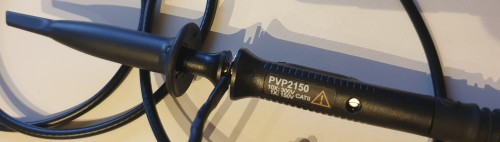
\includegraphics[height=3cm]{rigol-sonde.jpg}%
}
\hfill
\subfloat[Oscilloscope\label{fig:compensation-oscillo}]{%
	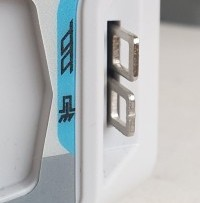
\includegraphics[height=3cm]{rigol-compensation-inputs.jpg}%
}
\caption{Points de réglage de la compensation (a) via la vis sur la sonde et (b) en connectant la sonde à l'oscilloscope.}
\label{fig:compensation}
\end{figure}

Branchez la sonde (crochet) sur l'attache supérieure de l'oscilloscope et la masse (pince) sur la partie inférieure.
L'oscilloscope entre automatiquement en mode « compensation » et vous affiche une onde carrée.

\Question{
À l'aide du petit tournevis en plastique fourni dans le kit, tournez la vis de la sonde jusqu'à obtenir un signal correctement compensé.
}
{
Les sondes sont habituellement correctement compensée d'usine, ça vaut la peine de chipoter un peu pour voir à quoi ressemble une sonde mal compensée.
Pour info, la datasheet de la sonde indique ceci :

\begin{center}
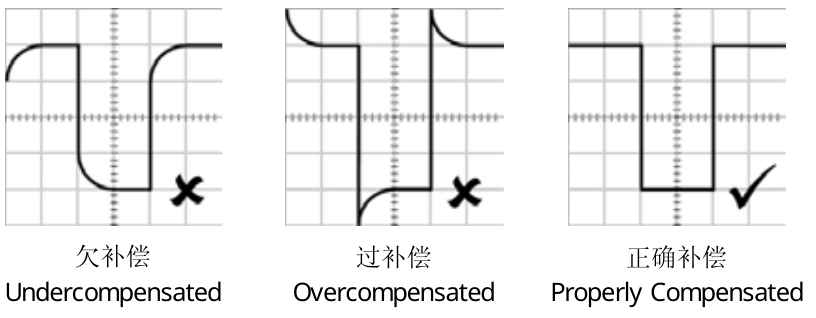
\includegraphics[width=.8\textwidth]{PV2150-compensation.png}
\end{center}
}






\section{Temps de propagation des signaux}
La sonde correctement configurée, vous allez pouvoir l'utiliser pour mesurer le temps de propagation d'un signal dans une porte logique \texttt{NOT}.
Vous avez deux modèles différents sur lesquels vous effectuerez les mêmes mesures : le \texttt{CD4069UB} et le \texttt{SN74LS04N}, tous deux de Texas Instrument\footnote{Les datasheets sont notamment disponibles sur Claco.}.
Le premier utilise une technologie CMOS tandis que le second exploite des transistors bipolaires.
Vous utiliserez une alimentation $V_{CC}$ (ou $V_{DD}$) de 5~V dans les deux cas.

\Question{
Pour chaque modèle, identifiez le temps de propagation renseigné par le fabricant.
\begin{astuce}
Attention à ne pas confondre temps de \textit{propagation} et temps de \textit{transition}.
Le constructeur indique clairement leur différence via des chronogrammes dans la datasheet du composant.
Pouvez-vous expliquer la différence ?
\end{astuce}
}
{
	Le temps de \textbf{propagation} est le temps nécessaire pour passer d'un niveau logique à 50\% en entrée à 50\% en sortie. On l'indique généralement par $t_{PLH}$ ou $t_{PHL}$.

	Le temps de \textbf{transition} est le temps nécessaire pour passer d'un niveau logique à 10\% à 90\% (ou l'inverse) sur l'entrée \textit{ou} la sortie. On l'indique généralement par $t_{TLH}$ ou $t_{THL}$.
	Cette dernière information n'est par exemple pas renseignée pour la famille \texttt{SN74} à base de bipolaires.

	Dans la datasheet du \texttt{SN74LS04N} on retrouve par exemple :
	\begin{center}
	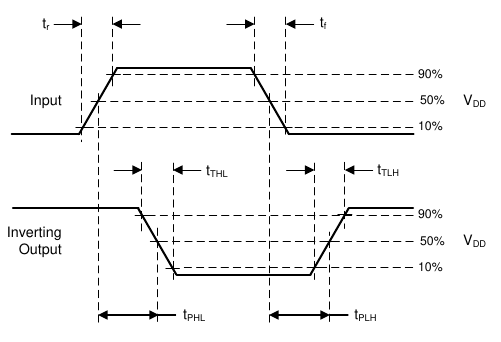
\includegraphics[width=.5\textwidth]{sn74ls04n-delays-graph.png}
	\end{center}


	\textbf{\texttt{SN74LS04N}} : $t_{PLH}$ = 9 ns (typ.) -- 15 ns (max), $t_{PHL}$ = 10 ns (typ) -- 15 ns (max)
	\textbf{\texttt{CD4069UB}} : $t_{PLH}$ = $t_{PHL}$ = 55 ns (typ.) -- 110 ns (max)

	
}



Vous allez à présent mesurer le temps de propagation de l'une de vos portes \texttt{NOT} à l'aide de l'oscilloscope.
À cette fin, vous allez brancher une sonde à la sortie de l'interrupteur et une seconde à la sortie de la porte logique.
Lorsqu'elle changera de l'état bas à l'état haut, vous pourrez observer l'écart entre les deux signaux qui est dû au délai de propagation du composant.

Voici le montage que vous devez réaliser :

\begin{center}
	\begin{circuitikz} \draw 

	(0,0) node [american not port] (not) {\footnotesize{\texttt{NOT}}}

	(-3,0) node[cute spdt mid arrow,xscale=-1] (sw) {}

	($(sw.out 1)-(1,0)$) node {\texttt{+5 V}} % 5V label
	(sw.out 1) node[rground, yscale=-1, rotate=-90] (alim) {} % 5V alim
	(sw.out 2) node [ground, rotate=-90] {} % ground

	(not.in 1) node[circle,fill,inner sep=1.5pt] () {}
	(not.in 1) to [bend left] ($(not.in 1)+(1,1)$) node [right] (chanA) {\texttt{Canal 1}}

	(sw.in) -- (not.in 1)

	(not.out) node[circle,fill, inner sep=1.5pt] () {}
	(not.out) to [bend right] ($(not.out)+(1,-0.5)$) node [right] (chanB) {\texttt{Canal 2}}
	(not.out) to [short] ($(not.out)+(0.5,0)$)

	;\end{circuitikz}
\end{center}

\Question{
Comment devez-vous régler le déclenchement (\textit{trigger}) de l'oscilloscope ?
}
{
	On va synchroniser la mesure sur l'entrée de la porte logique, l'origine du changement de niveau logique.
	Il s'agit du \textbf{canal 1} qui va passer de l'état bas (0 V) à l'état haut (5 V).
	Il faut régler le seuil de déclenchement sur une valeur intermédiaire qui n'est pas trop proche des extrémités pour éviter de déclencher la prise de mesure sur du bruit.
	Choisissons \textbf{2.5 V sur une pente montante}.

	Enfin, le type de déclenchement est une \textbf{capture unique} (single). On n'enregistre les échantillons que quand la condition de déclenchement est rencontrée, on remplit la mémoire et c'est fini.
}

\Question{\label{q:mesure-delai}
Effectuez la mesure en déplaçant l'interrupteur de 0 V à 5 V, provoquant le changement d'état de la sortie.
Mesurez le délai de propagation lorsque les signaux passent à 2.5~V.

	\begin{astuce}
		Veillez à utiliser les mêmes types de sonde pour les deux canaux afin de limiter les écarts de mesure.
	\end{astuce}
	\begin{astuce}
		Ne laissez pas les entrées inutilisées \textit{flottantes}, connectez-les à la masse ou à 5~V.
	\end{astuce}
}
{
	On devrait normalement obtenir des valeurs assez proches de celles renseignées dans les datasheets.

	Au sujet des entrées flottantes, TI a notamment écrit un rapport assez complet sur le sujet intitulé « \href{https://e2e.ti.com/cfs-file/__key/communityserver-discussions-components-files/151/4760.scba004c_5F00_slownfloatingCMOS.pdf}{Implications of Slow or Floating CMOS Inputs} ».
}

\Question{
	Quel est le plus petit intervalle de temps que vous pouvez mesurer avec l'oscilloscope Rigol \texttt{DS1104Z-Plus} dans la configuration utilisée ?
}
{
	Étant donné qu'on utilise deux canaux, le taux d'échantillonnage est de 500~MS/s. La résolution temporelle est donc de 2~ns.
}

\Question{
	À la lumière de ces résultats, critiquez la pertinence de votre mesure à la question~\ref{q:mesure-delai}.
}
{
	Pour le \texttt{SN74LS04N}, on a moins d'un ordre de grandeur entre la résolution temporelle et la durée mesurée. Il serait de bon ton de trouver une alternative pour obtenir une mesure plus précise.
}

\Question{
	En supposant les délais de propagation identiques entre les différentes portes logiques d'un même package, connectez quatre portes \texttt{NOT} en série et calculez le temps de propagation moyen à l'aide d'une nouvelle mesure.

	\begin{center}
		\begin{circuitikz} \draw 
	
		(0,0) node [american not port] (or) {\footnotesize{\texttt{NOT}}}
	
		(-3,0) node[cute spdt mid arrow,xscale=-1] (sw) {}
	
		($(sw.out 1)-(1,0)$) node {\texttt{+5 V}} % 5V label
		(sw.out 1) node[rground, yscale=-1, rotate=-90] (alim) {} % 5V alim
	
		(or.in 1) node[circle,fill,inner sep=1.5pt] () {}
		(or.in 1) to [bend left] ($(or.in 1)+(1,1)$) node [right] (chanA) {\texttt{Canal 1}}
	
		(sw.out 2) node [ground, rotate=-90] {} % ground
		(sw.in) -- (or.in 1)

		(or.out) node [american not port, anchor=in 1] (or2) {\footnotesize{\texttt{NOT}}}
		(or2.out) node [american not port, anchor=in 1] (or3) {\footnotesize{\texttt{NOT}}}
		(or3.out) node [american not port, anchor=in 1] (or4) {\footnotesize{\texttt{NOT}}}
	
		(or4.out) node[circle,fill, inner sep=1.5pt] () {}
		(or4.out) to [bend left] ($(or4.out)+(1,+1)$) node [right] (chanB) {\texttt{Canal 2}}
		(or4.out) to [short] ($(or4.out)+(0.5,0)$)
		;\end{circuitikz}
	\end{center}
}{}


\Question{
	Comment évolue ce délai en fonction de la charge capacitive ?
	Observez la différence entre la sonde en x1 et en x10.
}
{
	Les datasheets indiquent que le délais doit augmenter.
	On peut simuler une charge capacitive différente en jouant avec la sonde : le réglage x10 devrait avoir une charge capacitive plus faible que la x1.
}

\section{Relevé de la caractéristique I-V d'une diode}

La diode est un composant non-linéaire~: le courant la traversant évolue non-linéairement par rapport à la tension qui lui est appliquée (voir figure~\ref{fig:diode-carac}).
L'oscilloscope est capable d'afficher l'évolution du signal sur un canal en fonction d'un autre grâce au mode «~X-Y~»\footnote{Le mode X-Y se cache dans le menu de la base temporelle de l'oscilloscope.}.
Il est donc possible d'utiliser un canal pour relever la tension appliquée à ses bornes et un second canal pour mesurer le courant qui la traverse.
L'oscilloscope ne mesurant que des tension, il s'agira de mesurer la tension aux bornes de la résistance de série et de la convertir mathématiquement en courant.

\begin{figure}[!h]
\centering
\subfloat[Caractéristique\label{fig:diode-circuit}]{%
	\shorthandoff{:!}
		\begin{circuitikz}\draw
			(0,3) to [american voltage source, l=$V_{dc}$] (0,0)
			(0,3) to [european resistor, l^=$100 \Omega$] (3,3)
			to [D] (3,0) -- (0,0)
		;\end{circuitikz}
	\shorthandon{:!}
}
\hspace*{2cm}
\subfloat[Circuit\label{fig:diode-carac}]{%
	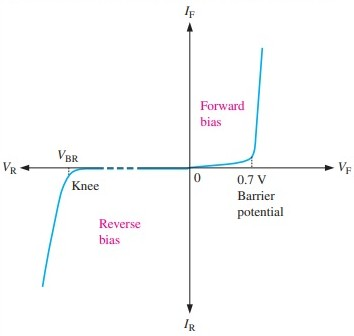
\includegraphics[width=.4\textwidth]{Voltage-Current-Characteristic-of-Diode.jpg}%
}
\caption{Caractéristique et circuit simple incorporant une diode.}
\label{fig:diode}
\end{figure}

\Question{
	Comment allez-vous configurer le générateur de signal ?
}
{
	Il faut un signal qui varie dans le temps. L'idéal est un signal triangulaire pour avoir une progression linéaire de la tension en fonction du temps.
	L'amplitude devrait être suffisamment large pour atteindre la tension de seuil, $5 V_{PP}$ est un bon début.
}

\Question{
	Réalisez le circuit (figure~\ref{fig:diode-circuit}) à l'aide d'une LED rouge, d'une diode \texttt{1N4007} ou une diode Zener ayant $V_z < 3 V$.
	Relevez ensuite le caractéristique I-V de la diode sélectionnée.
	\begin{astuce}
		Rappelez-vous que l'oscilloscope prend ses mesures référencées à la masse. Placez donc la résistance intelligemment pour pouvoir prendre la mesure à ses bornes.
	\end{astuce}
}
{
	Dans la figure~\ref{fig:diode-circuit}, il faut inverser la diode et la résistance en série pour pouvoir prendre la tension aux bornes de la diode à l'aide de l'oscilloscope.
	Le canal 1 est branché en parallèle de la source de tension, le canal 2 sur la résistance.
	Si le mode X-Y n'affiche qu'un seul point au lieu de la caractéristique entière, vérifier l'échelle temporelle qui est peut-être trop basse.

	La LED rouge est sympa pour avoir quelque chose qui clignote (si la fréquence de la source est suffisamment basse), la 1N4007 supporte de relativement gros courants (1 A sans soucis) et à donc moins de chance de mourir dans l'opération, la diode Zener est intéressante pour observer l'avalanche sur la caractéristique. Dans ce dernier cas, la tension $V_z < 3$ est importante puisque le générateur utilisé ne peut aller au-delà de 10 $V_{PP}$ ; une tension d'avalanche relativement faible nous laisse de la marge pour observer l'évolution du courant négatif dans la Zener.
}

\section{Tracé de courbe de Bode}
L'oscilloscope \texttt{DS1104Z-Plus} est capable d'afficher l'évolution de statistiques et mesures au cours du temps, comme par exemple une tension moyenne, un rapport de cycle ou une fréquence.
En réglant le générateur de signal pour effectuer un balayage en fréquence (\textit{sweep}), il devient possible de suivre l'évolution du comportement d'un filtre en fonction de la fréquence du signal d'entrée.

\begin{figure}[h!]
	\centering
	\begin{circuitikz} \draw
	(0,0)
	 node[ground]{}
	to[american voltage source, v=$V_{in}$, invert] (0,3)
	to[R, l=$R$] (3,3)
	(3,0) to[C, l=$C$, v=$V_{out}$] (3,3)
	(3,0)--(0,0);
	\end{circuitikz}
\caption{Filtre RC passe-bas.}
\label{fig:filtre-rc}
\end{figure}

\Question{
	Réalisez le filtre passe-bas proposé à la figure~\ref{fig:filtre-rc} en utilisant des composants de valeur arbitraire.
	Déterminez théoriquement la fréquence de coupure $f_c$ du filtre que vous venez de réaliser.
}
{
	$f_c = \frac{1}{2\pi\cdot RC}$
}

\Question{
	Configurez le générateur de signal pour qu'il effectue un balayage en fréquence depuis $f_c/10$ jusqu'à $10\cdot f_c$.
	Observez l'évolution de la forme de $V_{out}$ en fonction du temps à l'oscilloscope.
}
{}

\Question{
	Configurez le relevé graphique de mesure pour afficher l'évolution de l'amplitude de $V_{out}$ pour les différentes fréquence.
}
{}







\section{Mesure de résistance à quatre fils}
Mesurer une résistance très faible devient compliqué avec un multimètre classique : la résistance des sondes elles-mêmes ne devient plus négligeable.
Pour s'affranchir de cette dernière, il est possible de réaliser une mesure à quatre fils.


\Question{
	Mesurez la valeur de la résistance à l'aide d'un multimètre.
	La valeur obtenue vous semble-t-elle cohérente ?
}
{
	On peut s'attendre à ce que l'ordre de grandeur soit correct, mais il est fort probable qu'on mesure $1.6\Omega$ au lieu de $1\Omega$.
	En fonction de la résistance utilisée, l'écart peut s'expliquer par la tolérance du fabricant, mais normalement on devrait être au-delà de cette dernière.
}

\Question{\label{q:r4fils-montage}
	En vous aidant de la configuration proposée au cours, déterminez le montage à réaliser pour mesurer précisément la valeur d'une résistance de $1\Omega$.
}
{
	Il faut une alimentation et deux multimètres.
	L'alimentation envoie un courant continu dans la résistance que le premier multimètre mesure précisément.
	Le second multimètre se place en parallèle de la résistance afin de déterminer la tension à ses borne.
	On a ensuite $R = V/I$.
}

\Question{
	À l'aide de ce montage, déterminez la valeur précise de la résistance.
	Prenez bien note de votre \textbf{protocole expérimental} (pourquoi, quoi et comment) afin que la prise de mesure soit reproductible.

	\textbf{Attention :} Veillez à ne pas dépasser la puissance maximale de votre résistance. Dans le doute, considérez qu'il s'agit d'une 1/4 W.
}
{
	\begin{description}
		\item[Pourquoi ?] Lorsqu'on tente de mesurer une résistance très faible ($<10\Omega$), la résistance des sondes n'est plus négligeable. Il convient alors d'utiliser une méthode alternative dans laquelle ces dernières n'interviennent plus. Bien que la valeur de la résistance est indiqué sur son corps, on pourrait se trouver dans une situation dans laquelle on souhaite mesurer la résistance d'un composant non -standard (fil, inductance, etc.).
		Note : On remarque que le pourquoi, comme souvent, correspond à l'énoncé initial.
		\item[Quoi ?] Mesure de la résistance via la mesure de courant et de tension.
		\item[Comment ?] Il s'agit du montage de la question~\ref{q:r4fils-montage}.
	\end{description}
}

\section{Analyse du contenu fréquentiel des signaux}
En plus des opérations mathématiques de base (addition, soustraction, etc.), l'oscilloscope est aussi capable d'appliquer une transformée de Fourier rapide (FFT) afin de décomposer le signal mesuré en une somme de sinusoïdes dont les fréquences sont des multiples entier de la fréquence fondamentale du signal.
Il affiche alors ce résultat sous la forme d'un graphe représentant l'amplitude du signal en fonction de différentes fréquences.

Ce mode est notamment utile pour vérifier le \textit{contenu fréquentiel} d'un signal et donc sa potentielle déformation.
Une sinusoïde parfaite ne contient qu'une seule fréquence tandis qu'une sinusoïde écrêtée, par exemple, aura un contenu fréquentiel beaucoup plus riche.

\Question{
	Connectez directement le générateur de signal à l'oscilloscope et relevez la FFT des différentes formes de signal que le générateur est capable de générer.
}
{
	Sinusoïde (fréquence fondamentale uniquement, mais on observe quelques harmonique de très faible amplitude néanmoins), triangle (quelques harmoniques impaires), carré (énormément d'harmoniques, jusqu'à relativement haute fréquence) et bruit (contenu fréquentiel homogène).
}

À l'aide d'un amplificateur opérationnel \texttt{LM741}, réalisez un montage inverseur de gain 10 alimenté en 0/5 V.

\Question{
	Relevez la FFT de $V_{out}$ lorsque le montage ne sature \textbf{pas}.
}
{
	On devrait retrouver une belle sinusoïde, mais on peut s'attendre à un certain contenu fréquentiel d'entrée de jeu.

	L'alimentation asymétrique est pour faciliter le montage en n'utilisant qu'une seule alimentation.
	Il faut du coup bien penser à décaler le signal d'entrée afin que ses deux bornes soient dans l'intervalle des alimentation 0/5 V.
}

\Question{
	Relevez la FFT de $V_{out}$ lorsque le montage sature.
}
{
	Ici on peut jouer avec le degré de saturation pour constater l'enrichissement progressif du contenu fréquentiel.
}

% => Jouer avec les différentes fenêtre de filtrage numérique.

\section{Condensateur mystère}
Il peut arriver qu'on doive déterminer la valeur d'un composant sans se référer aux informations du constructeur.
Dans cette partie, vous avez une condensateur de capacité inconnue.

\Question{
	Sans utiliser de multimètre, déterminez la capacité du condensateur.
	Établissez clairement votre protocole expérimental.
}
{
	Il est possible de déterminer la valeur de la capacité en la plaçant dans un filtre d'ordre 1 avec une résistance connue. La fréquence de coupure indique univoquement la capacité.

	Il est aussi possible de mesurer le temps de charge de ce même circuit RC.

	\begin{center}
		\begin{tabular}{|c|c|c|c|c|c|c|c|c|c|}
		1 		& 2 		& 3 			& 4 		& 5 		& 6 		& 7 			& 8 	& 9 			& 10 \\
		\hline
		10 nF & 4.7 nF & 6.8 nF & 470 nF & 47 nF & 56 nF & 4.7 µF & 1 µF & 2.2 µF & 33 µF \\
		\end{tabular}
	\end{center}
}


\section{Vérification des caractéristiques des sondes x1/x10}
Dans un monde parfait, l'impédance de la sonde est constante et élevée afin de réduire son effet de charge (son influence sur le montage).
Nous ne vivons pas dans un monde parfait, en atteste les informations du fabricant de la sonde en figure~\ref{fig:probe-input-impedance}.

\begin{figure}[h!]
\centering
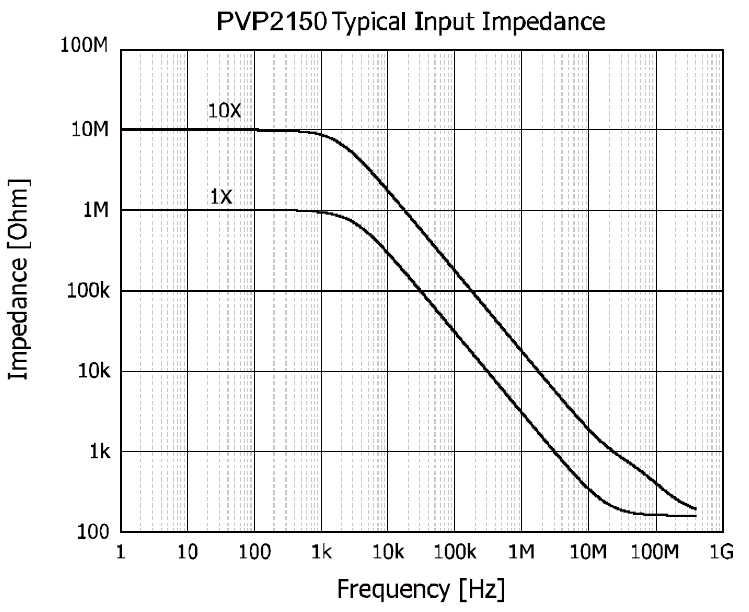
\includegraphics[width=.7\textwidth]{PVP2150_input-impedance.png}
\caption{Évolution de l'impédance de la sonde en fonction de la fréquence du signal mesuré.}
\label{fig:probe-input-impedance}
\end{figure}

Dans cette partie, vous allez vérifier l'évolution de l'impédance de la sonde en fonction de la fréquence du signal mesuré.

\Question{
	Réalisez un montage diviseur de tension :
	\begin{center}
		\begin{circuitikz} \draw
			(0,0)
			 node[ground]{}
			to[american voltage source, v=$V_{in}$, invert] (0,3)
			to[C, l=$1 k\Omega$] (3,3)
			(3,0) to[R, l=$100 k\Omega$, v=$V_{out}$] (3,3)
			(3,0)--(0,0);
		\end{circuitikz}
	\end{center}
	Réglez l'amplitude de la tension d'entrée à 2 $V_{PP}$.
	Vérifiez que le signal n'est pas atténué en sortie à une fréquence de 100 Hz.

	\begin{astuce}
		Vérifiez la valeur des résistances, n'ayez pas une confiance aveugle dans les tiroirs de rangements du labo.
	\end{astuce}
}
{ On le vérifie bien, on trouve $V_{out} \approx 1V$ d'amplitude, le diviseur impédant ayant un rapport de 100/101.}

\Question{
	Vérifiez l'évolution de l'impédance des sondes en faisant varier la fréquence du signal d'entrée.
	Vérifiez que l'impédance de celle-ci est bien plus élevée en mode x10.
	\begin{astuce}
		Si vous utilisez une sonde \texttt{PVP2150} pour le générateur, vous pouvez la laisser en mode x1.
	\end{astuce}
}
{
	En faisant un petit montage diviseur de tension avec deux résistances de 100 $k\Omega$ et un signal d'entrée de 1 V d'amplitude, on est censé obtenir 500 mV en sortie.
	Avec l'augmentation de la fréquence, on observe que l'amplitude de la sortie diminue.
	Par exemple, à 100 kHz on a environ 230 mV, soit une atténuation supplémentaire de 50\% qui correspond à l'impédance de la sonde qui est passée sous 100 $k\Omega$ en mode x1 à cette fréquence.
	En passant la sonde en mode x10 à cette même fréquence, on trouve que $V_{out}$ est remontée à 460 mV qui correspond bien à une augmentation de l'impédance de la sonde.

	Voici par exemple le comportement de la sonde x1 entre 1 Hz et 100 kHz en progression logarithmique.
	\begin{center}
	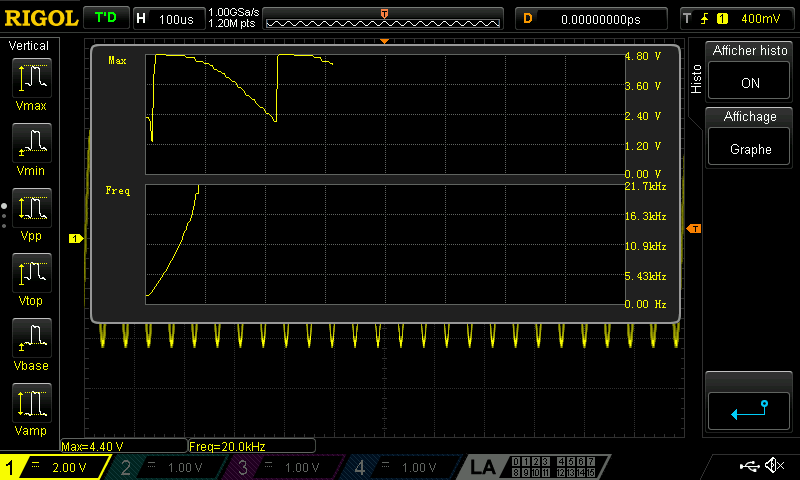
\includegraphics[width=.8\textwidth]{DS1Z_probex1_sweep_1Hz_100kHz_log.png}
	\end{center}
}



% \section{Prise de mesure différentielle}
% => Prendre une différence de potentiel au milieu du montage, faire bon usage des canaux mathématiques afin d'afficher la différence entre les deux sondes. Demander quels sont les avantages (pas besoin de sonde active) et désavantages (on divise par deux le taux d'échantillonnage, différence mathématique qui dépend de la qualité de la conversion numérique, pas de rejet du mode commun) de cette méthode par rapport à une vraie mesure différentielle.

\end{document}
